\section{مقدمه}

در بخش \ref{sec:mri-basics}
 توضیح داده شد که چرا تصویر برداری \mri طولانی و احتیاج به سپری شدن زمان دارد. برای کاهش این زمان باید یا میدان مغناطیسی و اندازه گرادیان ها را افزایش داد و یا از تعداد نمونه های مورد پردازش کاست. از آنجا که افزایش میدان مغناطیسی علاوه بر خطراتی که دارد، از لحاظ مهندسی نیز کار ساده ای نیست، روش هایی که مبتنی بر کاهش تعداد نمونه ها هستند اهمیت بیشتری پیدا کرده اند.
 
 

\begin{figure}[t]
	\centering
	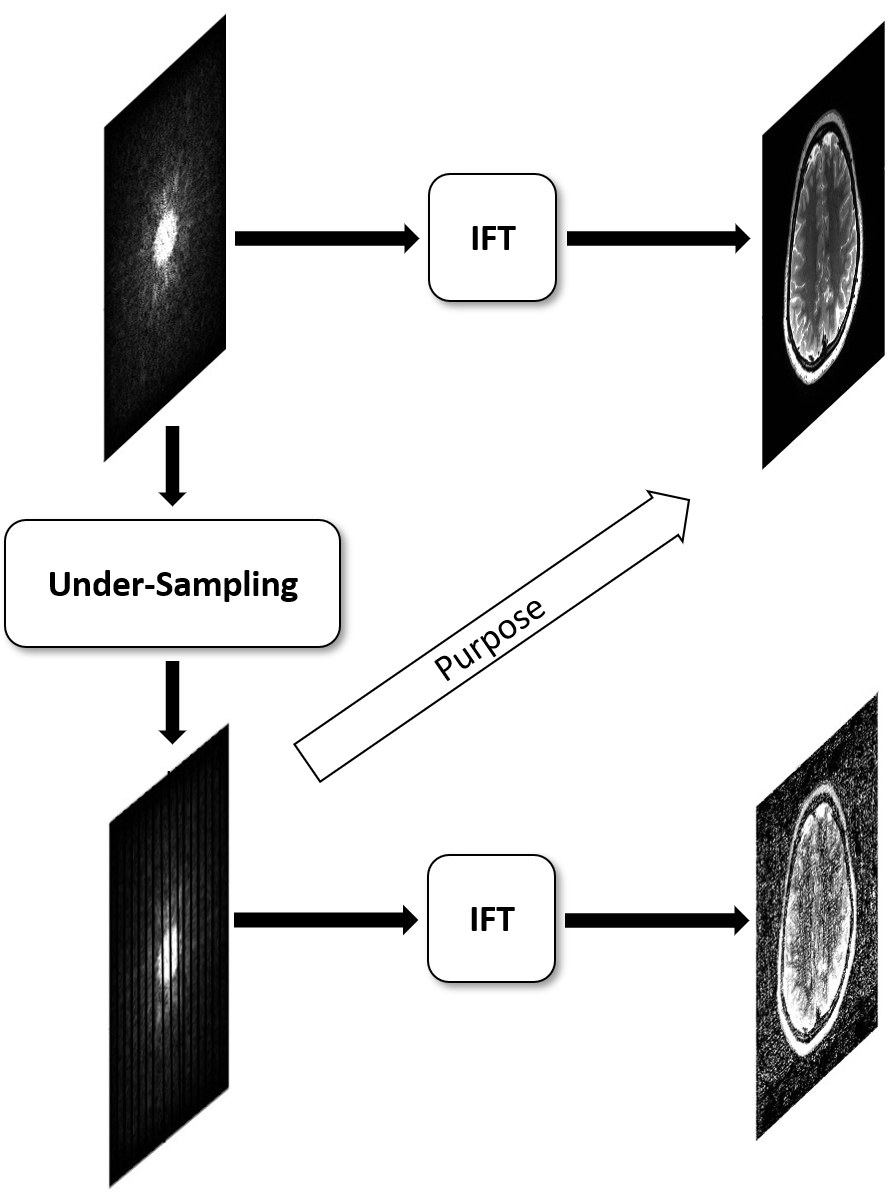
\includegraphics[width=0.3\linewidth]{chapters/chapter-3/figs/purpose-diagram}
	\caption{}
	\label{fig:purpose-diagram}
\end{figure}

 به طور کلی، می‌توان هدف این گونه پردازش ها را در شکل \ref{fig:purpose-diagram}، مشاهده نمود. سعی بر آن است که داده های مورد پردازش را کاهش داد. در اثر این اقدام، تصویر باز سازی شده دچار تداخل
 \LTRfootnote{Aliasing}
می‌شود. اما هدف این گونه پردازش ها این است که این مشکلات ایجاد نشود و تصویری با همان کیفیت، ایجاد شود.  

برای این هدف، باید از اطلاعاتی اضافی در بازسازی تصاویر استفاده کرد. در بخش پردازش های سیگنالی از این حقیقت استفاده می‌شود که تصاویر ما حقیقی هستند و در بخش تصویربرداری موازی، از اطلاعات سیم پیچ های مختلف استفاده می‌کنند. اما در بخش حسگری فشرده و یادگیری عمیق از اطلاعات خود تصویر به گونه ای استفاده می‌شود تا کیفیت آن کاهش پیدا نکند. 
















